\section{Diagrammi - Framework}

\begin{figure}[H]
	\centering
	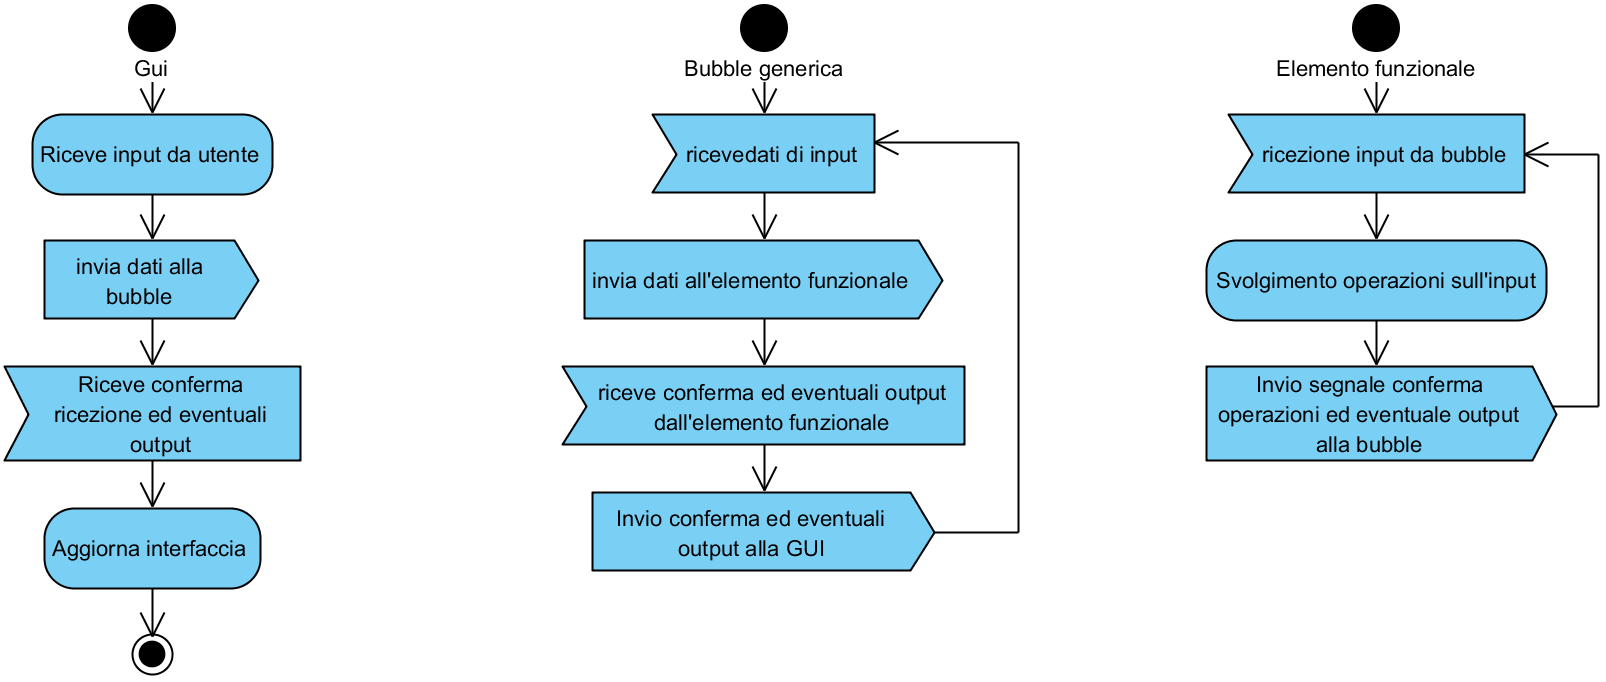
\includegraphics[width=14cm]{diagrammi_img/attivita/framework.png}
	\caption{Diagramma di attività - Aggiunta elemento alla To-do list}
	\label{fig:alt_framework}
\end{figure}

\begin{figure}[H]
	\centering
	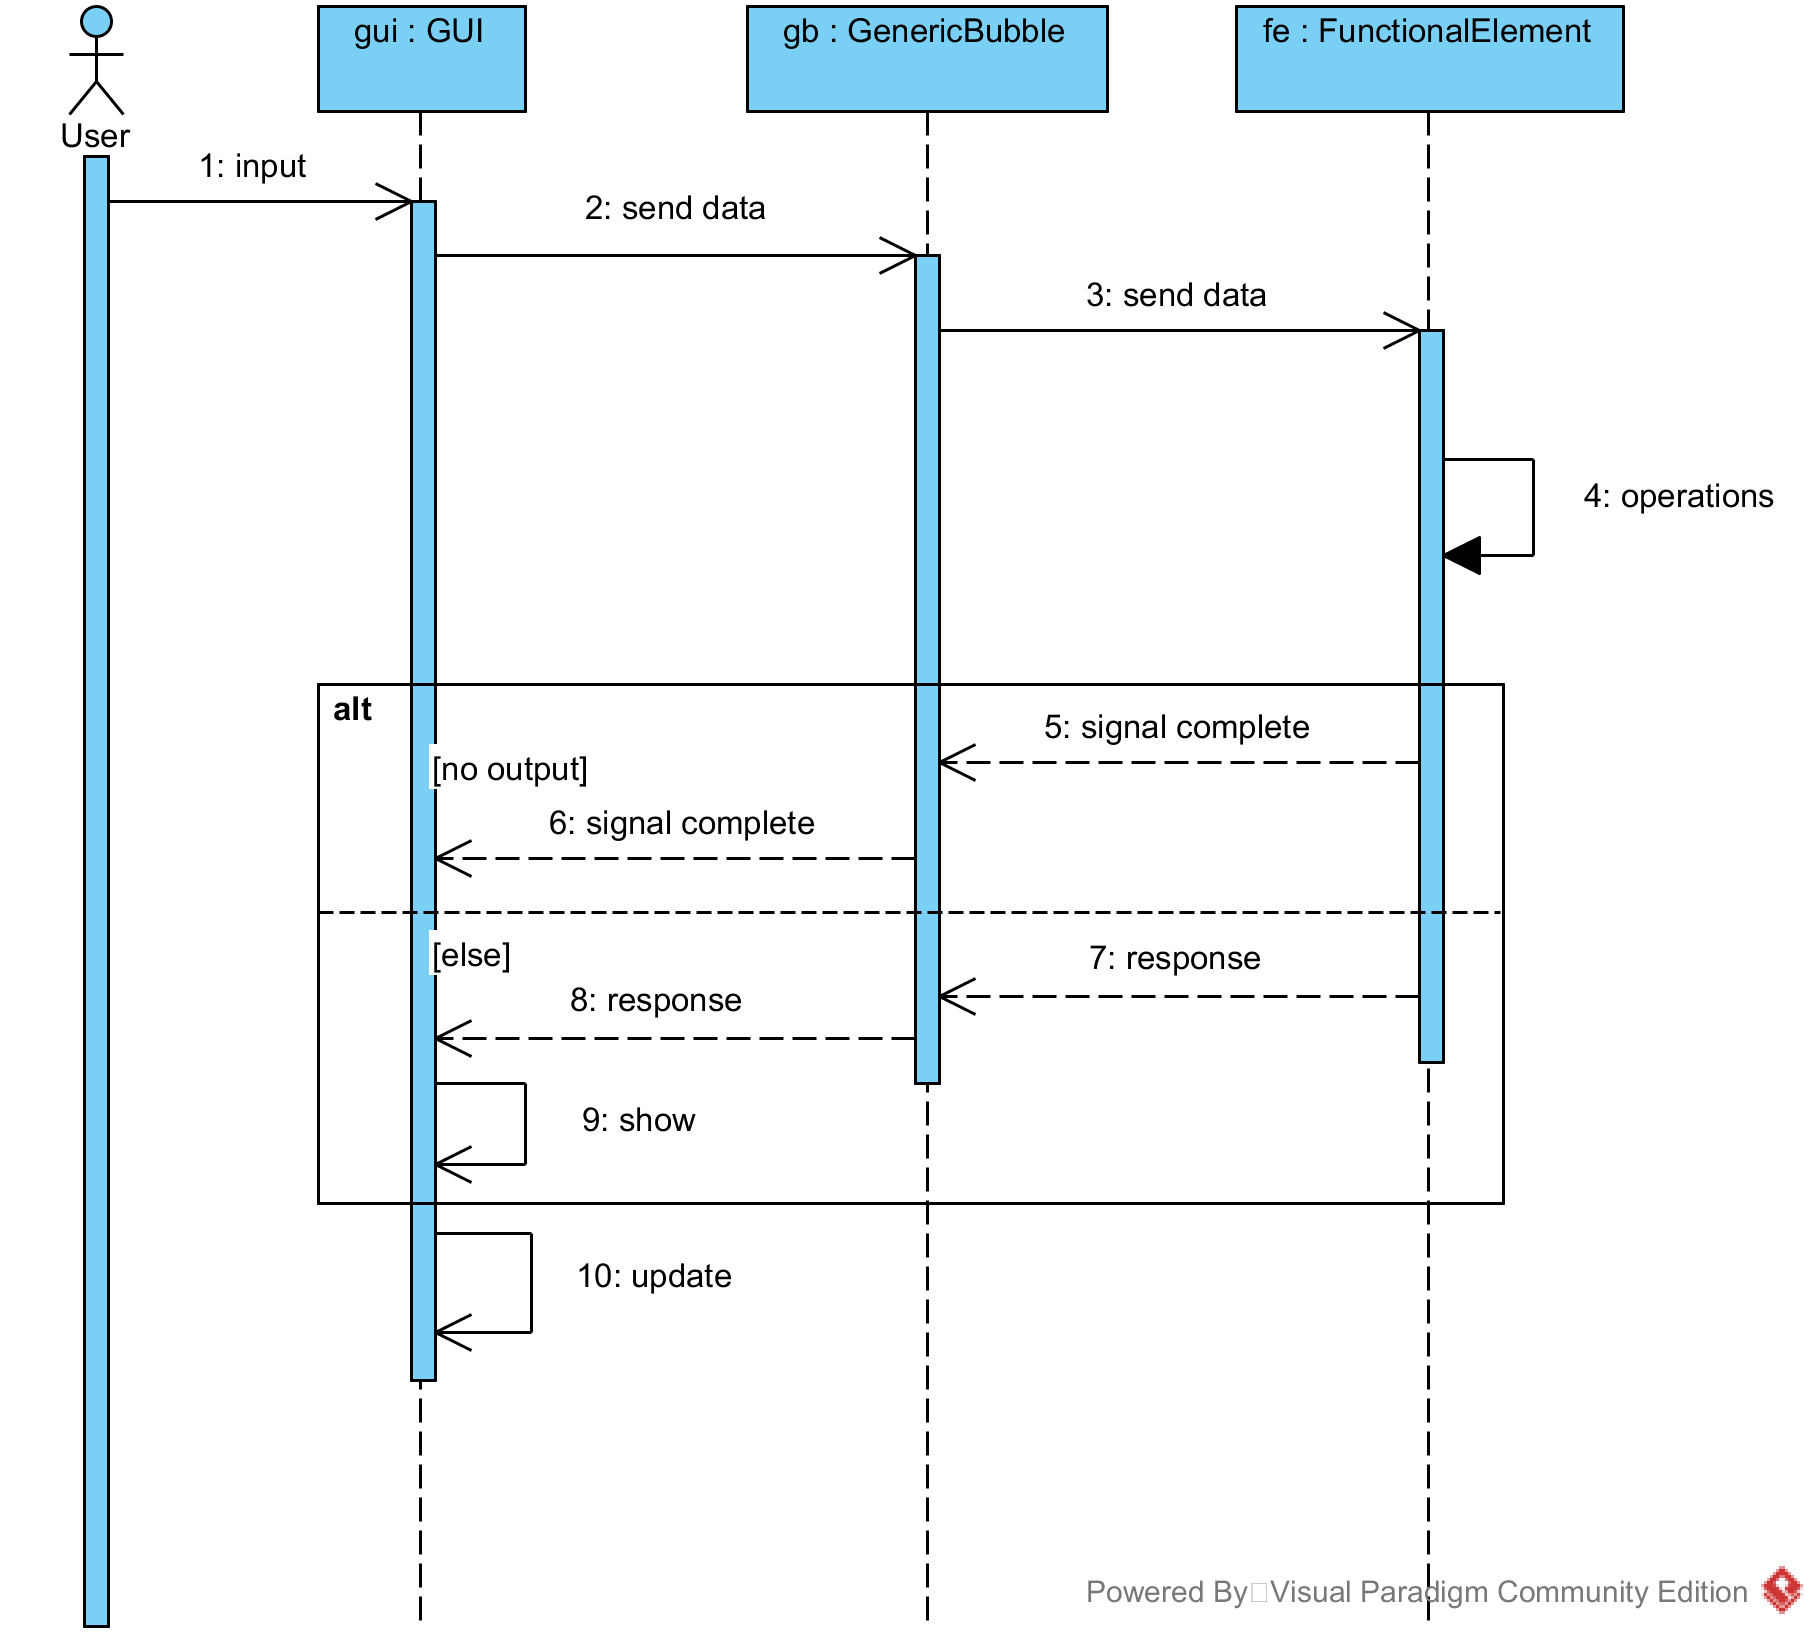
\includegraphics[width=14cm]{diagrammi_img/sequenza/framework.png}
	\caption{Diagramma di sequenza - Framework}
	\label{fig:seq_framework}
\end{figure}

Nei digrammi \ref{fig:alt_framework} e \ref{fig:seq_framework} sono rappresentate le interazioni che avvengono generalmente e ad alto
livello tra le componenti del framework, model, view e controller. I segnali inviati dall’utente
vengono ricevuti dalla view, la quale li invia al controller; questo quindi individua l’elemento
funzionale incaricato di elaborare le informazioni e quindi gli inoltra i dati. L’elemento funzionale
del model compie le operazioni richieste e ritorna una risposta o un segnale di conferma a seconda
sia richiesto dell’output. La risposta (o segnale) ricevuto dal controller viene quindi rispedita
alla view, che mostrerà all’utente l’esito della sua richiesta ed eventuali informazioni ricevute.